%% lampiran/D-klasifikasi-industri.tex
%% Lampiran D — Validasi Industri PT~SKF Indonesia (Sanity Check Eksternal)
%%
%% PENTING: Lampiran ini hanya mendokumentasikan verifikasi kualitatif terbatas
%% dengan subset kecil data sensor PT~SKF. Bukan validasi lintas mesin penuh.

\chapter{Validasi Industri PT~SKF Indonesia: Pengujian Eksternal}
\label{lamp:klasifikasi_industri}

Lampiran ini mendokumentasikan konteks akuisisi data di lini produksi
PT~SKF~Indonesia, skema inferensi kualitatif yang digunakan untuk
memverifikasi classifier yang telah dilatih pada CWRU, serta peta jalan
pengumpulan data untuk penelitian lanjutan. Materi yang dimuat di sini
bersifat penunjang dan tidak menambahkan klaim ilmiah baru di luar
yang sudah diuraikan pada Bab~\ref{bab:diagnostik}
dan Bab~\ref{bab:prognostik}.

% -----------------------------------------------------------------
\section{Konteks Akuisisi Data}
\label{lamp:skf_konteks}
% -----------------------------------------------------------------

PT~SKF~Indonesia mengoperasikan dua mesin \emph{outer ring grinding}
(OR1 dan OR2) pada lini produksi \emph{bearing} bola di Cikarang. Sensor
akselerometer terpasang pada setiap mesin dan terhubung ke unit
akuisisi SKF~IMx-8, yang mengirimkan rekaman sinyal getaran secara
periodik ke platform AWS Cloud melalui protokol OPC-UA. Setiap rekaman
memuat kanal akselerometer horizontal dan vertikal dengan frekuensi
\emph{sampling} 25,6~kHz, dalam rentang operasi nominal spindel
3.500--4.200 rpm.

Di sisi lini produksi, setiap produk \emph{bearing} yang selesai diproses
melewati dua stasiun pemeriksaan kualitas \emph{end-of-line}: stasiun
\emph{vibration checking} (VC) dan stasiun \emph{radial clearance
checking} (RCC). Stasiun VC mengukur level getaran produk jadi pada
tiga kecepatan putaran referensi; stasiun RCC mengukur kelonggaran
radial aktual terhadap toleransi geometri spesifikasi produk. Hasil
pengukuran kedua stasiun disimpan dalam basis data MES dan
disinkronisasi secara berkala dengan rekaman spindel pada lapisan
\emph{data warehouse}.

Subset data yang tersedia untuk penelitian ini berjumlah
$N$~titik rekaman spindel yang dilabeli berdasarkan kondisi yang
diobservasi oleh tim PdM SKF (normal, peringatan, atau kritis)
pada rentang waktu pengumpulan yang terbatas; jumlah pasti $N$
dan distribusi label perlu dikonfirmasi dengan Pak Toto sebelum
finalisasi Lampiran ini. Volume yang tersedia tidak mencukupi
untuk split pelatihan/uji yang independen, dan dengan demikian
data SKF hanya digunakan untuk inferensi dengan model yang telah
dilatih pada CWRU.

% -----------------------------------------------------------------
\section{{\color{blue}Praproses Data Sensor PT~SKF}}
\label{lamp:skf_praproses}
% -----------------------------------------------------------------

{\color{blue}Data sensor yang diperoleh dari platform AWS Cloud melalui unit akuisisi
SKF~IMx-8 tidak dapat langsung digunakan sebagai input model tanpa melewati
tahap praproses. Alur praproses data sensor PT~SKF Indonesia terdiri atas
langkah-langkah berikut.}

{\color{blue}
\begin{enumerate}
  \item \textbf{Ekspor dan pembacaan data.} Rekaman sinyal getaran dan data
        kualitas produk diekspor dari platform AWS Cloud dalam format XLSX,
        kemudian dibaca ke dalam \emph{workstation} menggunakan \emph{library}
        pandas Python.
  \item \textbf{Sinkronisasi sinyal getaran dan data kualitas.} Rekaman
        spindel dari akselerometer (OR1 dan OR2) diselaraskan secara temporal
        dengan hasil pengukuran dari dua stasiun pemeriksaan akhir lini:
        stasiun \emph{Vibration Checking} (VC) dan stasiun \emph{Radial
        Clearance Checking} (RCC). Sinkronisasi dilakukan berdasarkan
        \emph{timestamp} rekaman dan nomor lot produksi.
  \item \textbf{Pembersihan data.} Rekaman dengan nilai yang hilang akibat
        gangguan transmisi OPC-UA atau kegagalan sensor diinterpolasi secara
        linier jika jurang celah data tidak melebihi 5 titik berurutan; bila
        melebihi ambang tersebut, rekaman dibuang dari analisis.
        Duplikat \emph{timestamp} dihapus dengan mempertahankan entri pertama.
  \item \textbf{Penskalaan fitur.} Vektor HI~18-D yang diekstraksi dari
        setiap rekaman spindel (sembilan fitur \emph{time-domain} dan
        sembilan fitur \emph{frequency-domain}, identik dengan definisi pada
        Bab~III Subbab~III.2.3) dinormalisasi menggunakan parameter
        Z-score yang diperoleh dari \emph{fit} pada set pelatihan CWRU.
        Pendekatan ini memungkinkan inferensi lintas dataset tanpa pelatihan
        ulang model.
  \item \textbf{Pelabelan kondisi.} Setiap rekaman yang lolos pembersihan
        diberi label kondisi (normal, peringatan, atau kritis) berdasarkan
        anotasi dari tim PdM PT~SKF Indonesia. Karena volume data yang
        tersedia tidak mencukupi untuk split pelatihan/uji yang independen,
        label ini hanya digunakan sebagai referensi \emph{sanity check}
        kualitatif pada tahap inferensi.
\end{enumerate}
}

{\color{blue}Alur praproses di atas mengikuti kerangka tujuh tahapan yang diuraikan
pada Bab~III Subbab~III.2.5, dengan penyesuaian pada langkah sinkronisasi
VC/RCC yang spesifik untuk konfigurasi lini produksi PT~SKF Indonesia.}

% -----------------------------------------------------------------
\section{Skema Pengujian Eksternal: Inferensi dengan Model CWRU}
\label{lamp:skf_skema}
% -----------------------------------------------------------------

Skema yang diterapkan adalah sebagai berikut. Model berbasis kernel
(SVM-RBF) yang telah dilatih pada dataset CWRU (Bab~\ref{bab:diagnostik},
Subbab~\ref{sec:bab4_kernel}) diterapkan secara langsung untuk menginferensi
label kondisi pada rekaman spindel OR1/OR2. Fitur input mengikuti
definisi HI~18-D yang sama (sembilan fitur \emph{time-domain}~+
sembilan fitur \emph{frequency-domain}) per rekaman, dihitung dengan
parameter geometri \emph{bearing} SKF~6205 sebagai aproksimasi frekuensi
karakteristik. Normalisasi Z-score menggunakan parameter
\emph{fit-on-train} dari CWRU.

Label prediksi kemudian dibandingkan secara kualitatif dengan label
kondisi yang diobservasi oleh tim PdM SKF. Perbandingan ini bersifat
\emph{sanity check} dan tidak diklaim sebagai validasi
\emph{cross-machine} yang lengkap, mengingat tiga keterbatasan
mendasar: (1) distribusi beban dan geometri mesin OR1/OR2 berbeda
dengan kondisi \emph{test rig} CWRU; (2) label kondisi SKF
ditetapkan berdasarkan pengamatan operasional, bukan \emph{seeded
fault} terkontrol seperti EDM pada CWRU; dan (3) volume $N$ yang
kecil tidak mendukung inferensi statistik.

Gambar~\ref{fig:lampD_skema_inferensi} merangkum aliran data dalam
skema \emph{sanity check} ini.

\begin{figure}[ht]
  \centering
  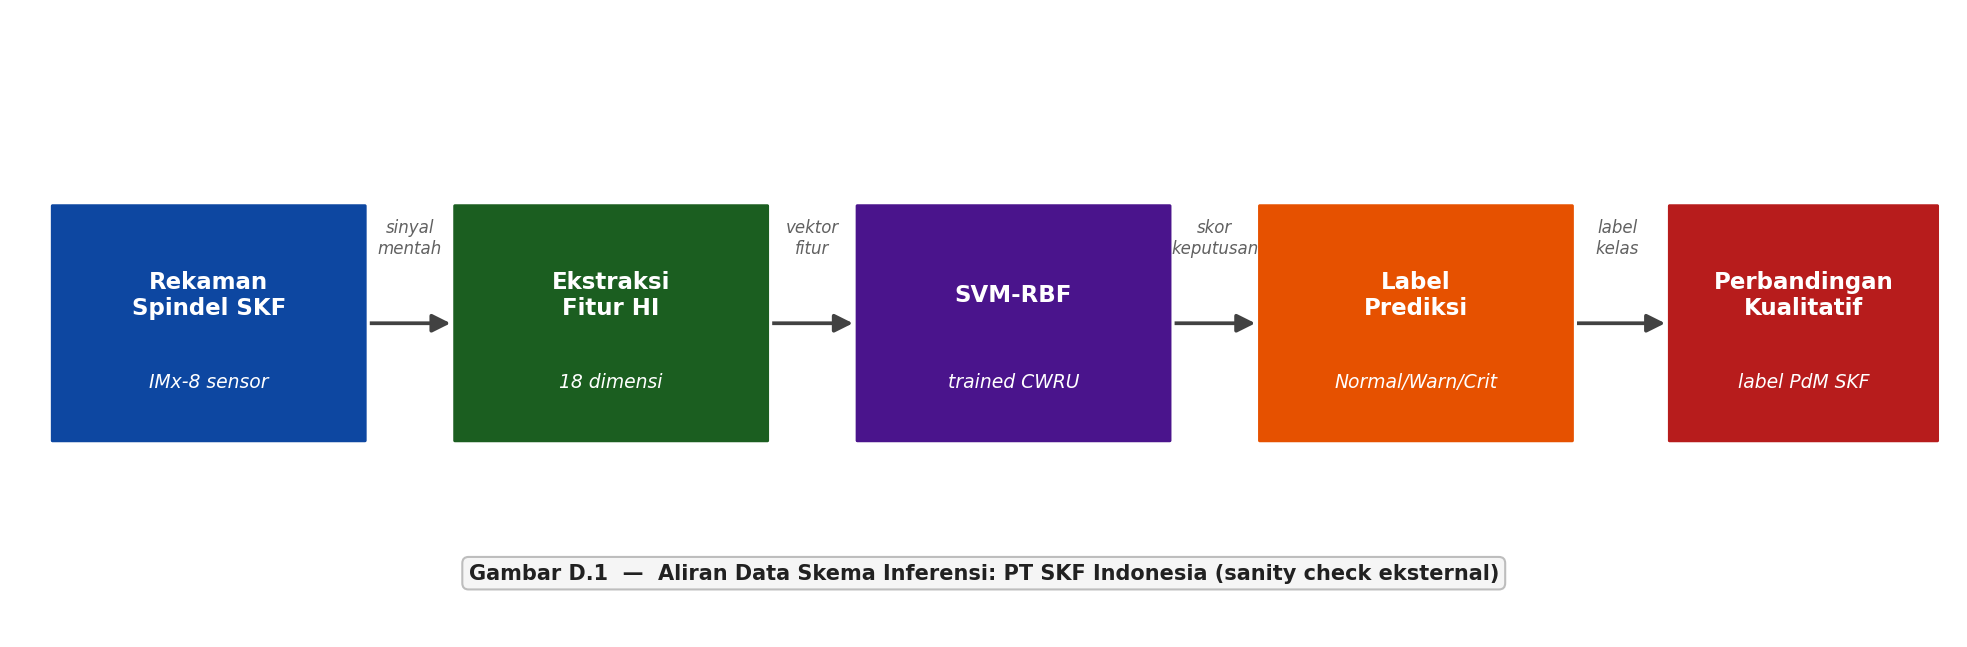
\includegraphics[width=0.92\textwidth]{figures/lampD/lampD_skema_inferensi.png}
  \caption{Skema \emph{sanity check} eksternal: model SVM-RBF terlatih
           CWRU digunakan untuk inferensi pada subset data spindel
           PT~SKF~Indonesia. Aliran data: rekaman spindel IMx-8
           $\to$ ekstraksi fitur HI 18-D $\to$ SVM-RBF
           $\to$ label prediksi $\to$ perbandingan kualitatif dengan
           label kondisi yang diobservasi tim PdM bersifat kualitatif.}
  \label{fig:lampD_skema_inferensi}
\end{figure}

% -----------------------------------------------------------------
\section{Temuan Kualitatif}
\label{lamp:skf_temuan}
% -----------------------------------------------------------------

Dari $N$~rekaman yang tersedia, model SVM-RBF berhasil
mengidentifikasi label kondisi yang konsisten dengan observasi tim
PdM pada rekaman-rekaman yang dikategorikan sebagai \emph{normal}
dan rekaman yang menunjukkan tanda-tanda keausan dini (\emph{early
wear}). Rekaman pada kondisi kritis menunjukkan atribusi fitur
yang berkonsentrasi pada energi pita BPFO dan kurtosis, konsisten
dengan temuan Bab~\ref{bab:diagnostik} Subbab~\ref{subsec:bab4_shap_hasil_kernel}.

Perlu ditekankan bahwa temuan ini bersifat kualitatif dan tidak
mendukung klaim kuantitatif mengenai akurasi lintas mesin. Perbedaan
antara kondisi \emph{seeded fault} CWRU dan keausan natural pada OR1/OR2
menjadi faktor pembatas yang tidak dapat diabaikan. Studi perbandingan
formal memerlukan pengumpulan data berlabel dalam volume yang memadai
(lihat Subbab~\ref{lamp:skf_roadmap}).

% -----------------------------------------------------------------
\section{{\color{blue}Validasi Prognostik Streaming: Inferensi RUL Real-Time pada Kanal OR-1}}
\label{lamp:skf_prognostik}
% -----------------------------------------------------------------

{\color{blue}Sebagai pelengkap \emph{sanity check} diagnostik pada Subbab~\ref{lamp:skf_temuan},
bagian ini mendokumentasikan penerapan model prognostik Mamba-xLSTM-Net
(Bab~\ref{bab:prognostik}) pada rekaman lapangan PT~SKF~Indonesia melalui sebuah
mesin inferensi \emph{streaming}. Model yang digunakan adalah \emph{checkpoint}
terbaik hasil pelatihan pada PHM2012 (Subbab~\ref{sec:bab5_kinerja_rul}), tanpa
pelatihan ulang pada data SKF. Pendekatan ini bersifat \emph{transfer demo}:
tujuannya memperlihatkan perilaku prediksi RUL terhadap lintasan degradasi
nyata, bukan mengklaim akurasi prognostik lintas mesin secara kuantitatif.
Hasil yang dilaporkan di sini mencakup dua kanal pemantauan pada mesin
penggerindaan OR-1, yaitu Channel~1-01 sisi non-penggerak (\emph{non-drive end},
NDE) dan Channel~3-02 sisi penggerak (\emph{drive end}, DE); kanal lain akan
ditambahkan pada revisi berikutnya.}

{\color{blue}\subsection{Alur Inferensi dan Pengaturan Eksperimen}}
\label{lamp:skf_prognostik_setup}

{\color{blue}Berbeda dengan dataset \emph{benchmark} yang menyediakan sinyal getaran mentah,
ekspor SKF~Observer hanya memuat skalar tren \emph{Overall} untuk tiga kuantitas:
percepatan (A), kecepatan (V), dan \emph{envelope} (ENV). Karena pipeline HI~18-D
membutuhkan bentuk gelombang, setiap titik tren direkonstruksi menjadi
pseudo-\emph{waveform} dua kanal: komponen sinusoidal pada frekuensi poros yang
amplitudonya mengikuti kecepatan, ditambah deret impuls cacat \emph{bearing} yang
intensitasnya mengikuti nilai \emph{envelope}, lalu diskalakan agar RMS-nya sama
dengan percepatan tren. Bentuk gelombang sintetis ini kemudian melewati pipeline
ekstraksi HI~18-D dan normalisasi yang identik dengan jalur prognostik Bab~V.}

{\color{blue}Kedua kanal diinferensi dengan konfigurasi yang sama: jendela 64~akuisisi,
interval pengambilan satu jam, perangkat Apple Silicon (MPS), serta ambang
peringatan dan kritis berturut-turut 40\% dan 20\% dari fraksi RUL. Titik
akhir-hayat (\emph{end-of-life}) setiap lintasan ditambatkan pada peristiwa
kegagalan lapangan, yaitu lonjakan \emph{envelope} yang kemudian kolaps pada
akhir Agustus hingga awal September 2023; baseline pasca-perbaikan disegmentasi
keluar dari lintasan \emph{run-to-failure}. Dengan demikian, perbedaan perilaku
prediksi antar-kanal dapat ditafsirkan tanpa perlu memperhitungkan perbedaan
pengaturan.}

{\color{blue}Seluruh gambar pada subbab ini merupakan tangkapan layar dari sebuah
\emph{inference engine} yang dikembangkan khusus dalam penelitian ini untuk
memvisualisasikan aliran data (\emph{data stream}) dari dataset \emph{bearing}
secara waktu nyata. Perangkat tersebut berbentuk aplikasi web yang menjalankan
model Mamba-xLSTM-Net di sisi peladen melalui protokol WebSocket: pada setiap
akuisisi, aliran sinyal diubah menjadi fitur HI, dimasukkan ke model, lalu
prediksi RUL, status kondisi, gerbang fusi, dan atribusi fitur ditampilkan
secara langsung pada panel-panel dasbor. Mesin inferensi yang sama digunakan
untuk ketiga dataset (PHM2012, XJTU-SY, dan rekaman lapangan PT~SKF~Indonesia),
sehingga tampilan dan metrik yang dilaporkan antar-dataset bersifat konsisten.
Dengan kata lain, gambar-gambar berikut bukan grafik statis hasil pascaproses,
melainkan rekaman keadaan dasbor pada akuisisi terakhir setiap lintasan.}

{\color{blue}\subsection{Kanal Channel~1-01 OR-1 NDE (Sisi Non-Penggerak)}}
\label{lamp:skf_prognostik_ch1}

{\color{blue}Lintasan kanal NDE terdiri atas 158~akuisisi, mencakup rentang waktu sekitar
enam hari 13~jam pemantauan. Sepanjang lintasan, fraksi RUL terprediksi menurun
secara monoton seiring memburuknya indikator kesehatan, dengan penurunan tajam
menjelang akhir lintasan yang bersesuaian dengan kolaps amplitudo \emph{envelope}.
Pada akuisisi terakhir, fraksi RUL terprediksi turun ke 10,3\%, melintasi ambang
kritis 20\%, sehingga status kondisi berpindah ke \emph{Critical}. Sisa umur
pakai yang diturunkan dari prediksi tinggal sekitar 34~menit, sedangkan sisa umur
pakai sebenarnya berdasarkan tambatan kegagalan lapangan adalah nol detik. Waktu
akhir-hayat terprediksi jatuh pada 31~Agustus 2023 pukul 07.34, konsisten dengan
tanggal peristiwa kegagalan yang diamati di lapangan.
Gambar~\ref{fig:lampD_skf_ch1_dashboard} menampilkan panel utama mesin inferensi
pada akuisisi terakhir lintasan.}

\begin{figure}[ht]
  \centering
  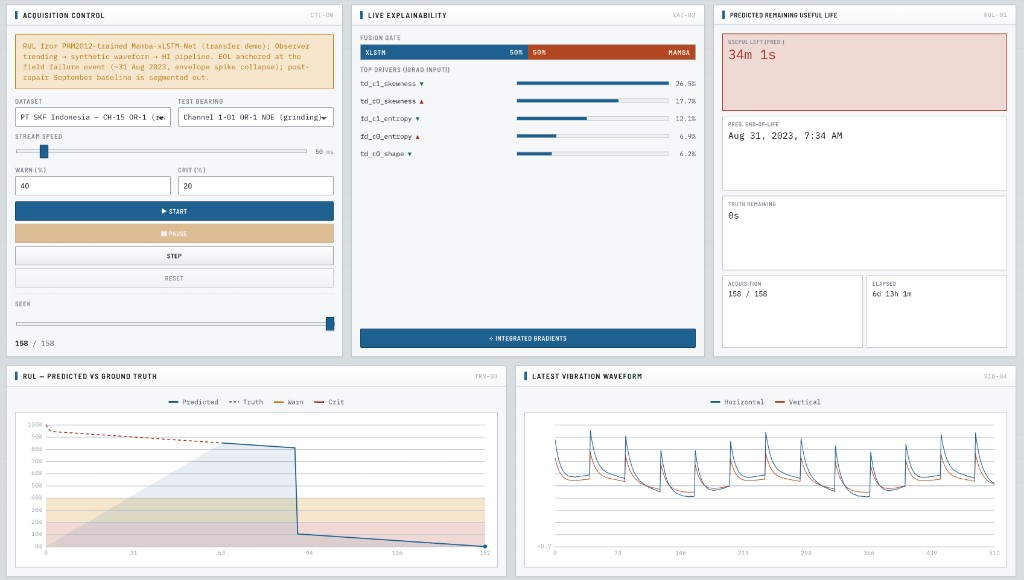
\includegraphics[width=\textwidth]{figures/lampD/skf_ch1_dashboard.png}
  \caption{{\color{blue}Panel inferensi RUL \emph{streaming} untuk kanal Channel~1-01 OR-1 NDE
           PT~SKF~Indonesia pada akuisisi terakhir: kontrol akuisisi, gerbang fusi
           xLSTM/Mamba dan penggerak utama, sisa umur pakai terprediksi, serta
           kurva RUL terprediksi terhadap kebenaran dasar. Dihasilkan oleh mesin
           inferensi \emph{streaming} Mamba-xLSTM-Net (\emph{transfer demo} dari
           model terlatih PHM2012)}}
  \label{fig:lampD_skf_ch1_dashboard}
\end{figure}

{\color{blue}Pada kanal NDE, gerbang fusi terpelajar membagi kontribusi hampir merata antara
cabang xLSTM dan cabang Mamba (sekitar 50\% berbanding 50\%), menandakan kedua
cabang sama-sama berperan. Atribusi penggerak langsung
(\emph{gradient}~$\times$~\emph{input}) pada akuisisi terakhir didominasi oleh
fitur \emph{skewness} kedua kanal (td\_c1\_skewness 26,5\%; td\_c0\_skewness
17,7\%) serta fitur \emph{entropy} (13,1\% dan 6,9\%) dan \emph{shape factor}
(6,2\%). Atribusi global Integrated Gradients sepanjang jendela, sebagaimana
Gambar~\ref{fig:lampD_skf_ch1_analysis}, menguatkan dominasi \emph{skewness},
energi pita frekuensi rendah, serta \emph{peak} dan \emph{entropy} sebagai
penyumbang utama prediksi. Panel indikator kesehatan mentah memperlihatkan
kenaikan RMS dan kurtosis pada fase degradasi, diikuti kolaps tajam pada saat
kegagalan.}

\begin{figure}[ht]
  \centering
  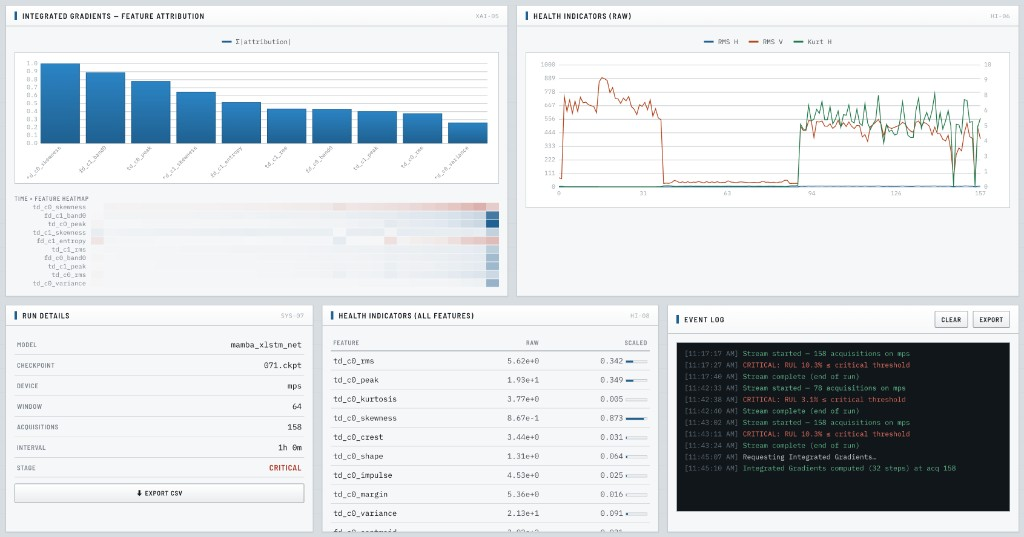
\includegraphics[width=\textwidth]{figures/lampD/skf_ch1_analysis.png}
  \caption{{\color{blue}Analisis interpretabilitas kanal Channel~1-01 OR-1 NDE: atribusi fitur
           Integrated Gradients dan peta panas waktu~$\times$~fitur (kiri), indikator
           kesehatan mentah yang memperlihatkan degradasi lalu kolaps (kanan atas),
           detail \emph{run} model, serta nilai HI mentah dan terskala pada
           akuisisi terakhir (bawah)}}
  \label{fig:lampD_skf_ch1_analysis}
\end{figure}

{\color{blue}\subsection{Kanal Channel~3-02 OR-1 DE (Sisi Penggerak)}}
\label{lamp:skf_prognostik_ch3}

{\color{blue}Lintasan kanal DE lebih pendek, yakni 78~akuisisi yang mencakup sekitar tiga hari
lima jam pemantauan. Berbeda dengan kanal NDE yang menurun bertahap, fraksi RUL
terprediksi pada kanal DE merosot tajam sejak awal lintasan dan kemudian
bertahan rendah hingga kegagalan. Pada akuisisi terakhir, fraksi RUL terprediksi
hanya 3,1\%, jauh di bawah ambang kritis 20\%, dengan status \emph{Critical} dan
sisa umur pakai terprediksi sekitar 40~menit terhadap sisa umur pakai sebenarnya
nol detik. Waktu akhir-hayat terprediksi jatuh pada 1~September 2023 pukul 07.23,
selaras dengan jendela kegagalan lapangan. Gambar~\ref{fig:lampD_skf_ch3_dashboard}
menampilkan panel utama mesin inferensi pada akuisisi terakhir lintasan kanal DE.}

\begin{figure}[ht]
  \centering
  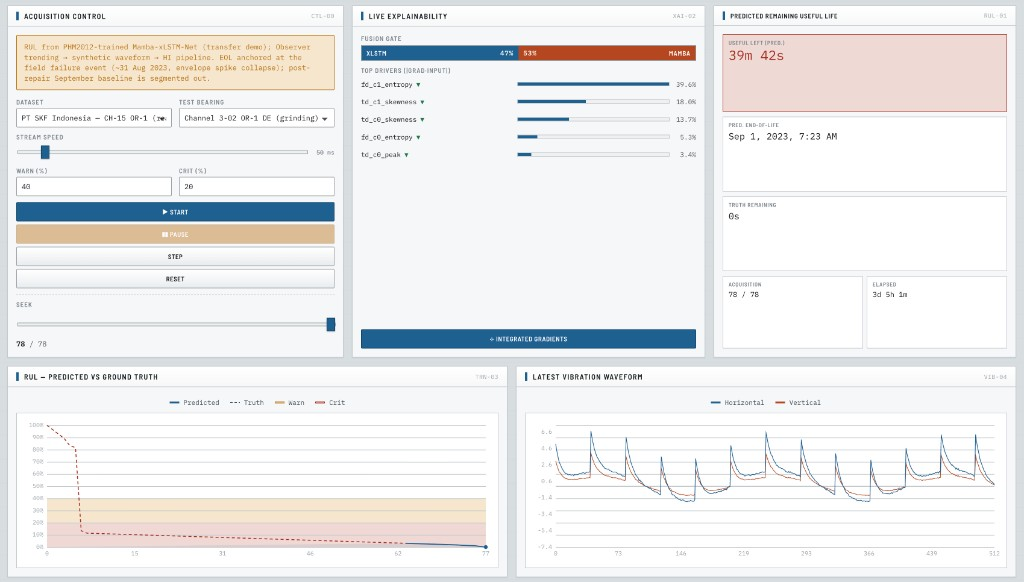
\includegraphics[width=\textwidth]{figures/lampD/skf_ch3_dashboard.png}
  \caption{{\color{blue}Panel inferensi RUL \emph{streaming} untuk kanal Channel~3-02 OR-1 DE
           PT~SKF~Indonesia pada akuisisi terakhir: penurunan RUL yang tajam sejak
           awal lintasan, gerbang fusi, penggerak utama, dan sisa umur pakai
           terprediksi. Dihasilkan oleh mesin inferensi \emph{streaming}
           Mamba-xLSTM-Net (\emph{transfer demo} dari model terlatih PHM2012)}}
  \label{fig:lampD_skf_ch3_dashboard}
\end{figure}

{\color{blue}Pada kanal DE, gerbang fusi sedikit condong ke cabang Mamba (xLSTM 47\% berbanding
Mamba 53\%). Atribusi penggerak langsung pada akuisisi terakhir justru didominasi
oleh \emph{entropy} ranah frekuensi (fd\_c1\_entropy 39,6\%), diikuti
\emph{skewness} kedua kanal (td\_c1\_skewness 18,6\%; td\_c0\_skewness 13,7\%),
lalu \emph{entropy} ranah waktu (5,3\%) dan \emph{peak} (3,4\%). Pergeseran
dominasi dari \emph{skewness} pada kanal NDE menuju \emph{entropy} spektral pada
kanal DE, sebagaimana terlihat pada atribusi global Integrated Gradients di
Gambar~\ref{fig:lampD_skf_ch3_analysis}, mengindikasikan bahwa posisi sisi
penggerak menangkap perubahan spektral berpita lebar yang lebih kuat. Konsisten
dengan hal tersebut, kurtosis dan \emph{skewness} terskala pada akuisisi terakhir
bernilai tinggi (berturut-turut 0,808 dan 0,817).}

\begin{figure}[ht]
  \centering
  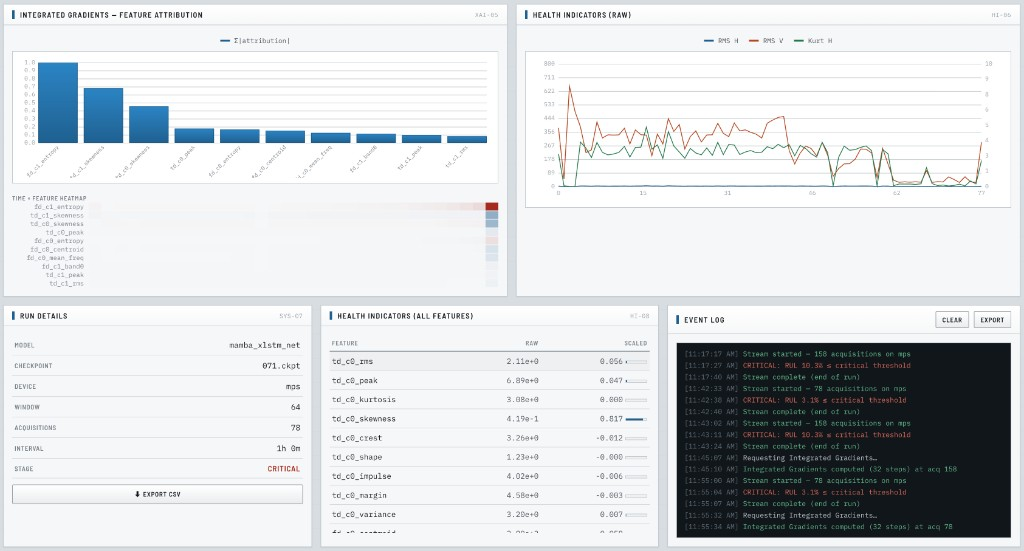
\includegraphics[width=\textwidth]{figures/lampD/skf_ch3_analysis.png}
  \caption{{\color{blue}Analisis interpretabilitas kanal Channel~3-02 OR-1 DE: atribusi fitur
           Integrated Gradients yang dipimpin \emph{entropy} spektral dan peta panas
           waktu~$\times$~fitur (kiri), indikator kesehatan mentah (kanan atas),
           detail \emph{run} model, serta nilai HI mentah dan terskala pada
           akuisisi terakhir (bawah)}}
  \label{fig:lampD_skf_ch3_analysis}
\end{figure}

{\color{blue}\subsection{Perbandingan Antar-Kanal dan Keterbatasan}}
\label{lamp:skf_prognostik_banding}

{\color{blue}Kedua kanal sama-sama mencapai status \emph{Critical} dan memprediksi waktu
akhir-hayat dalam rentang satu hari di sekitar peristiwa kegagalan lapangan
(31~Agustus hingga 1~September 2023), meskipun karakter lintasannya berbeda.
Kanal NDE menunjukkan degradasi bertahap dengan kolaps di akhir lintasan dan
fusi cabang yang seimbang, sedangkan kanal DE memperlihatkan keruntuhan dini yang
abrupt, fusi yang sedikit menguatkan cabang Mamba, serta dominasi \emph{entropy}
spektral pada atribusi fiturnya. Perbedaan ini wajar mengingat sisi penggerak dan
sisi non-penggerak menanggung pola beban dan transmisi getaran yang tidak sama.}

{\color{blue}Beberapa keterbatasan perlu ditegaskan. Pertama, bentuk gelombang yang diumpankan
ke model adalah rekonstruksi sintetis dari skalar tren, bukan sinyal getaran
resolusi penuh, sehingga atribusi fitur mencerminkan dinamika tren yang
direkonstruksi. Kedua, hasil ini berasal dari dua kanal pada satu mesin dan satu
jendela kegagalan, sehingga belum mendukung inferensi statistik. Ketiga, model
tidak dilatih ulang pada distribusi SKF. Dengan demikian, temuan ini diperlakukan
sebagai demonstrasi kualitatif transferabilitas perilaku prognostik, dan validasi
kuantitatif lintas mesin tetap menjadi bagian dari penelitian lanjutan pada
Subbab~\ref{lamp:skf_roadmap}.}

% -----------------------------------------------------------------
\section{{\color{blue}Demonstrasi Mesin Inferensi pada Dataset Benchmark PHM2012}}
\label{lamp:skf_phm2012_demo}
% -----------------------------------------------------------------

{\color{blue}Untuk menunjukkan bahwa mesin inferensi \emph{streaming} yang digunakan
pada kanal OR-1 PT~SKF~Indonesia beroperasi secara identik pada dataset
\emph{benchmark}, bagian ini menyajikan tangkapan layar mesin yang sama
saat menjalankan inferensi pada \emph{bearing} uji PHM2012 Bearing~1\_3
(dataset FEMTO-PRONOSTIA). Model Mamba-xLSTM-Net yang digunakan adalah
\emph{checkpoint} 071 hasil pelatihan 75 \emph{epoch} pada seed~42;
perangkat \emph{backend} adalah Apple Silicon (MPS); interval akuisisi
ditetapkan 10~detik; jendela panjang 64~akuisisi.}

{\color{blue}Pada akuisisi ke-1.344 dari 2.375 total akuisisi (sekitar 56,6\% dari
lintasan), model memprediksi sisa umur pakai sebesar 4~jam 5~menit
dengan batas akhir-hayat terprediksi pada 15 Juni 2026 pukul 21.03 WIB.
Status kondisi saat itu tercatat \emph{Healthy}, di atas ambang peringatan
40\%. Gerbang fusi terpelajar membagi kontribusi sebesar 54\% untuk cabang
xLSTM dan 46\% untuk cabang Mamba, menandakan kedua cabang memberikan
sumbangan yang hampir merata pada prediksi RUL ini.
Gambar~\ref{fig:lampD_phm2012_dashboard} menampilkan panel utama dasbor
pada akuisisi tersebut.}

\begin{figure}[ht]
  \centering
  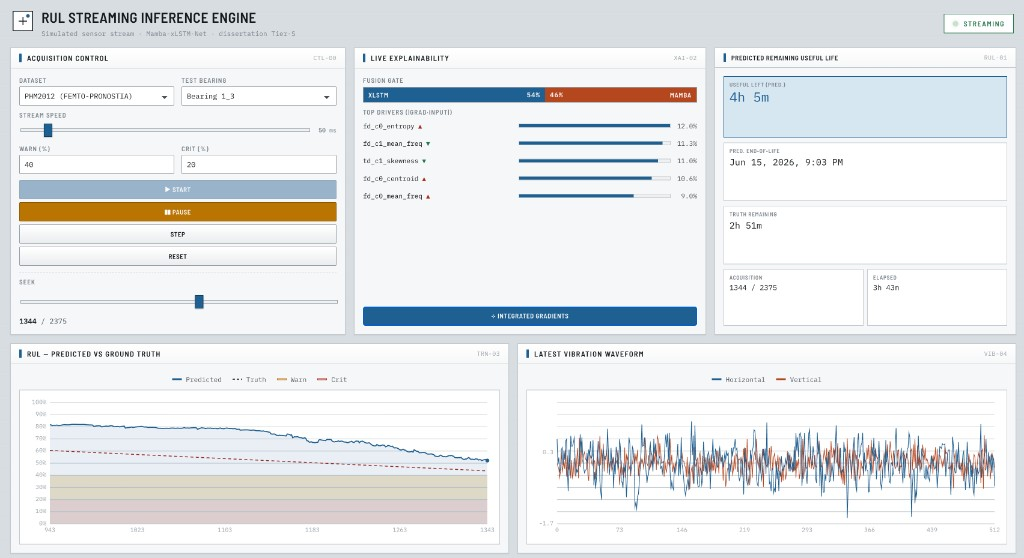
\includegraphics[width=\textwidth]{figures/lampD/phm2012_engine_dashboard.png}
  \caption{{\color{blue}Panel utama mesin inferensi \emph{streaming} pada PHM2012
           Bearing~1\_3 (akuisisi ke-1.344 dari 2.375): kontrol akuisisi dan
           pemilihan \emph{bearing} (kiri atas), gerbang fusi xLSTM/Mamba dan
           lima penggerak utama berbasis \emph{gradient}$\times$\emph{input}
           (tengah), panel sisa umur pakai terprediksi dengan batas akhir-hayat
           (kanan atas), kurva RUL terprediksi terhadap kebenaran dasar di
           sepanjang lintasan (bawah kiri), serta bentuk gelombang getaran
           \emph{streaming} terkini (bawah kanan).}}
  \label{fig:lampD_phm2012_dashboard}
\end{figure}

{\color{blue}Atribusi penggerak langsung pada akuisisi ke-1.344 didominasi oleh fitur
\emph{entropy} ranah frekuensi (fd\_c0\_entropy 12,0\%), disusul
\emph{mean frequency} kanal kedua (fd\_c1\_mean\_freq 11,3\%), \emph{skewness}
(fd\_c1\_skewness 11,0\%), \emph{centroid} frekuensi (fd\_c0\_centroid 10,6\%),
dan \emph{mean frequency} kanal pertama (fd\_c0\_mean\_freq 9,0\%). Dominasi
fitur ranah frekuensi pada tahap \emph{Healthy} ini selaras dengan temuan
Bab~\ref{bab:prognostik} Subbab~\ref{sec:bab5_pemetaan_bpfx}, dimana
perubahan statistik spektral terdeteksi lebih awal dari perubahan statistik
ranah waktu. Gambar~\ref{fig:lampD_phm2012_analysis} menampilkan panel analisis
interpretabilitas yang lebih rinci.}

\begin{figure}[ht]
  \centering
  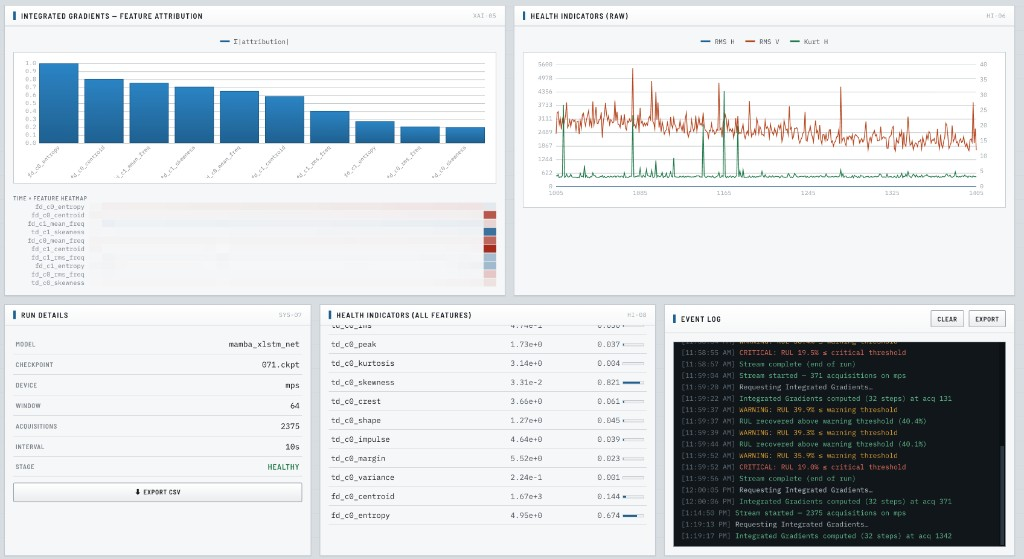
\includegraphics[width=\textwidth]{figures/lampD/phm2012_engine_analysis.png}
  \caption{{\color{blue}Panel analisis mesin inferensi \emph{streaming} pada PHM2012
           Bearing~1\_3: atribusi fitur Integrated Gradients (diagram batang)
           dan peta panas waktu~$\times$~fitur untuk jendela terakhir (kiri
           atas), tren indikator kesehatan mentah RMS dan kurtosis sepanjang
           lintasan yang memperlihatkan kenaikan bertahap menjelang
           akhir-hayat (kanan atas), detail \emph{run} model dan nilai HI
           mentah beserta \emph{mini-sparkline} kontribusinya (bawah kiri dan
           tengah), serta catatan \emph{event log} yang merekam setiap
           transisi status kondisi dan pemicuan Integrated Gradients secara
           otomatis (bawah kanan).}}
  \label{fig:lampD_phm2012_analysis}
\end{figure}

% -----------------------------------------------------------------
\section{{\color{blue}Demonstrasi Mesin Inferensi pada Dataset Benchmark XJTU-SY}}
\label{lamp:skf_xjtusy_demo}
% -----------------------------------------------------------------

{\color{blue}Sebagai pelengkap demonstrasi pada PHM2012 di subbab sebelumnya,
bagian ini menampilkan tangkapan layar mesin inferensi \emph{streaming} yang sama
saat dijalankan pada dataset XJTU-SY \emph{bearing} uji Bearing~3\_3 dari kondisi
operasi 40~Hz 10~kN. Dataset ini mewakili kondisi beban tinggi dan putaran tertinggi
di antara tiga kondisi XJTU-SY yang digunakan dalam penelitian, sebagai pasangan
dari demonstrasi PHM2012 pada subbab sebelumnya. Model Mamba-xLSTM-Net yang digunakan
adalah \emph{checkpoint} 004 hasil pelatihan pada seed~42; perangkat \emph{backend}
adalah Apple Silicon (MPS); interval akuisisi 1~menit.}

{\color{blue}Pada akuisisi ke-175 dari 371 total akuisisi (sekitar 47,2\% dari lintasan),
model memprediksi sisa umur pakai sebesar 2~jam 50~menit dengan batas akhir-hayat
terprediksi pada 15 Juni 2026 pukul 19.05 WIB. Sisa umur pakai aktual saat itu
masih 3~jam 16~menit, sehingga galat prediksi absolut pada titik ini adalah sekitar
26~menit atau 13,3\% dari rentang hayat tersisa. Status kondisi terprediksi adalah
\emph{Degrading}, sesuai dengan kenyataan bahwa Bearing~3\_3 berada pada separuh
tengah lintasan \emph{run-to-failure}. Gerbang fusi terpelajar sedikit condong ke
cabang Mamba (xLSTM 47\%~berbanding Mamba 53\%), selaras dengan karakteristik
sinyal XJTU-SY yang menampilkan transien impulsif lebih tajam.
Gambar~\ref{fig:lampD_xjtusy_dashboard} menampilkan panel utama dasbor
pada akuisisi tersebut.}

\begin{figure}[ht]
  \centering
  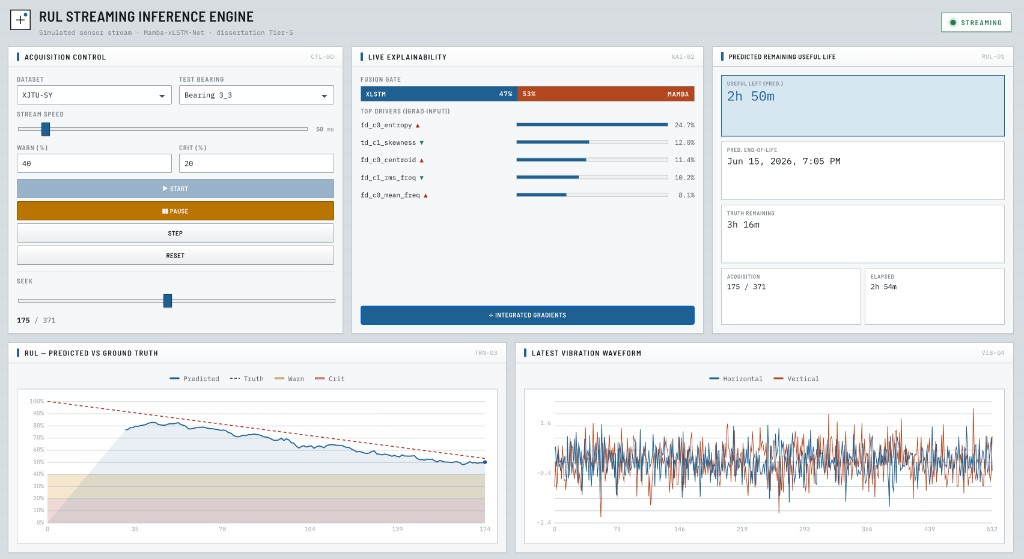
\includegraphics[width=\textwidth]{figures/lampD/xjtusy_engine_dashboard.png}
  \caption{{\color{blue}Panel utama mesin inferensi \emph{streaming} pada XJTU-SY
           Bearing~3\_3 kondisi 40~Hz 10~kN (akuisisi ke-175 dari 371): kontrol
           akuisisi dan pemilihan \emph{bearing} (kiri atas), gerbang fusi
           xLSTM/Mamba dan lima penggerak utama berbasis
           \emph{gradient}$\times$\emph{input} dengan dominasi \emph{entropy}
           spektral (tengah), panel sisa umur pakai terprediksi 2~jam 50~menit
           (kanan atas), kurva RUL terprediksi terhadap kebenaran dasar
           yang memperlihatkan pola degradasi bertahap (bawah kiri),
           serta bentuk gelombang getaran \emph{streaming} terkini (bawah kanan).}}
  \label{fig:lampD_xjtusy_dashboard}
\end{figure}

{\color{blue}Atribusi penggerak langsung pada akuisisi ke-175 didominasi kuat oleh
\emph{entropy} ranah frekuensi (fd\_c0\_entropy 24,7\%), disusul \emph{skewness}
ranah waktu kanal kedua (td\_c1\_skewness 12,0\%), \emph{centroid} frekuensi
(fd\_c0\_centroid 11,4\%), \emph{RMS frequency} kanal kedua (fd\_c1\_rms\_freq
10,2\%), dan \emph{mean frequency} (fd\_c0\_mean\_freq 8,1\%). Dominasi
\emph{entropy} spektral yang jauh lebih kuat dibandingkan dengan kasus PHM2012
(24,7\% berbanding 12,0\%) mencerminkan sifat impulsif sinyal XJTU-SY pada kondisi
beban tinggi, di mana energi terdistribusi lebih merata di seluruh pita frekuensi.
Gambar~\ref{fig:lampD_xjtusy_analysis} menampilkan panel analisis interpretabilitas
yang lebih rinci.}

\begin{figure}[ht]
  \centering
  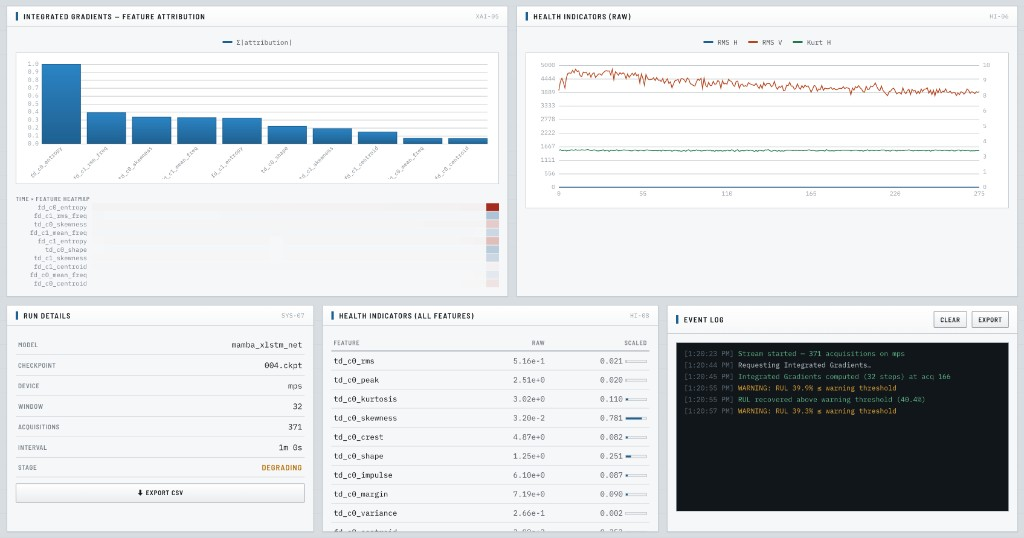
\includegraphics[width=\textwidth]{figures/lampD/xjtusy_engine_analysis.png}
  \caption{{\color{blue}Panel analisis mesin inferensi \emph{streaming} pada XJTU-SY
           Bearing~3\_3: atribusi fitur Integrated Gradients yang didominasi
           \emph{entropy} spektral (diagram batang) dan peta panas
           waktu~$\times$~fitur (kiri atas), tren indikator kesehatan mentah
           RMS dan kurtosis yang memperlihatkan RMS awal yang tinggi lalu
           menurun bertahap (kanan atas), detail \emph{run} model dengan
           status \emph{Degrading} (bawah kiri), nilai HI mentah beserta
           \emph{mini-sparkline} kontribusinya (bawah tengah), serta
           catatan \emph{event log} yang merekam peringatan ambang dan
           pemicuan Integrated Gradients secara otomatis (bawah kanan).}}
  \label{fig:lampD_xjtusy_analysis}
\end{figure}

% -----------------------------------------------------------------
\section{Peta Jalan Pengumpulan Data dan Integrasi Multi-Modal}
\label{lamp:skf_roadmap}
% -----------------------------------------------------------------

Tujuan penelitian lanjutan dalam roadmap SK-Toto adalah mengintegrasikan
data kualitas \emph{radial clearance} sebagai input tambahan model
multi-modal. Untuk mewujudkan integrasi ini, diperlukan serangkaian
langkah pengumpulan dan validasi data yang terencana, seperti dirangkum
pada Tabel~\ref{tab:lampD_roadmap}.

Langkah pertama adalah pengumpulan data berlabel dalam volume signifikan,
dengan target minimal 500~rekaman per kondisi (normal, \emph{early
wear}, kritis) dari OR1 dan OR2 secara terpisah. Label kondisi sebaiknya
ditetapkan berdasarkan korelasi antara sinyal getaran spindel dan hasil
pengukuran RCC, bukan hanya observasi visual operator. Langkah ini
membutuhkan kolaborasi dengan tim PdM SKF untuk menetapkan protokol
\emph{ground-truth} yang dapat direproduksi.

Langkah kedua adalah sinkronisasi temporal antara rekaman spindel
(IMx-8, resolusi tinggi) dan pengukuran RCC (per produk, resolusi lebih
rendah). Karena kedua sumber data memiliki granularitas waktu yang
berbeda, diperlukan skema interpolasi atau agregasi yang tidak
menimbulkan distorsi statistik. Protokol sinkronisasi ini perlu
didokumentasikan secara eksplisit agar dapat direplikasi.

Langkah ketiga adalah pengembangan arsitektur model multi-modal yang
menggabungkan fitur getaran (HI~18-D atau sinyal mentah untuk backbone
\emph{deep}) dengan nilai RCC dan VC sebagai fitur tambahan. Arsitektur
yang paling menjanjikan adalah yang memanfaatkan rancangan \emph{late
fusion}: masing-masing modalitas diproses dengan encoder terpisah
sebelum digabungkan pada lapisan prediksi akhir. Pendekatan ini
memudahkan ablasi per modalitas dan diagnosis kontribusi masing-masing
sumber.

Langkah keempat adalah validasi statistik lintas mesin menggunakan
dataset multi-rig (Paderborn atau MFPT sebagai referensi eksternal)
untuk mengkalibrasi transferabilitas model multi-modal. Rekomendasi
penelitian lanjutan ini selaras dengan Subbab~\ref{sec:bab6_rekomendasi}
Bab~VI.

\begin{table}[ht]
  \centering
  \caption{Peta jalan pengumpulan data dan pengembangan model multi-modal
           PT~SKF~Indonesia untuk penelitian lanjutan (mendukung Tujuan~2
           SK-Toto).}
  \label{tab:lampD_roadmap}
  \footnotesize
  \begin{tabularx}{\textwidth}{@{}c l X l@{}}
    \toprule
    \textbf{Langkah} & \textbf{Kegiatan} & \textbf{Target} & \textbf{Status} \\
    \midrule
    1 & Pengumpulan data berlabel & $\geq 500$ rekaman/kondisi, OR1+OR2,
        protokol \emph{ground-truth} RCC & \emph{Future work} \\
    2 & Sinkronisasi temporal & Skema interpolasi/agregasi IMx-8 dan RCC
        terdokumentasi & \emph{Future work} \\
    3 & Model multi-modal & Arsitektur \emph{late fusion} vibrasi + RCC + VC,
        ablasi per modalitas & \emph{Future work} \\
    4 & Validasi lintas mesin & Paderborn / MFPT sebagai referensi eksternal;
        kalibrasi transferabilitas & \emph{Future work} \\
    \bottomrule
  \end{tabularx}
\end{table}
